\documentclass[a4paper]{article}

\usepackage[english]{babel}
\usepackage[utf8]{inputenc}
\usepackage{amsmath}
\usepackage{graphicx}
\usepackage{float}
\restylefloat{table}

\title{Improvements and extensions on a Social Simulation.}

\author{prive}

\date{\today}

\begin{document}

\maketitle
\clearpage
\tableofcontents
\clearpage

\section{Introduction}
Short introduction here.

\clearpage

\section{Existing model}
About the existing NLogo simulation.

\subsection{Design}
Summary of how it is designed

\subsection{Simulation}
\label{sec:initialsim}
For the simulation, the following parameters were used for all experiments:
\begin{itemize}
\item Fine: $\$250$
\item Pedestrians: $50$
\item Pedestrian green time: $20$ ticks
\end{itemize}
As well as the following experiment-specific constraints:\\

\begin{tabular}{ r | l | l }
  Exp. & Cars & Car green time (ticks) \\
  \hline
  1 &  0 & 100 \\
  2 & 10 & 100 \\
  3 & 50 & 100 \\
  4 &  0 & 20  \\
  5 & 10 & 20  \\
  6 & 50 & 20  \\
\end{tabular}\\

Running the simulation for $100 000$ ticks, the results were the following:
\begin{table}[H]
\centering
\begin{tabular}{ l | c c c c }
  Police Presence Prob. & 0\% & 33\% & 66\% & 100\% \\ 
  \hline
  Experiment 1 & 3.92 & 2.40 & 0 & 0  \\
  Experiment 2 & 0.15 & 0.03 & 0 & 0  \\
  Experiment 3 & 0    & 0    & 0 & 0  \\
  Experiment 4 & 0.37 & 0    & 0 & 0  \\
  Experiment 5 & 0.15 & 0    & 0 & 0  \\
  Experiment 6 & 0    & 0    & 0 & 0  \\
\end{tabular}
\caption{Average number of times an adaptive 
pedestrian walks through a red light.}
\end{table}

We will reference these results in later chapters.

\clearpage

\section{Changes and their immediate effects}
Changes made to the model, why, and how they directly  affected the simulation.

\subsection{Viewing Distance}
We introduced a 'viewing range' for agents, where they would only be able to look ahead a fixed amount of $patches$ (for cars).

\subsubsection{Motivation}
In the existing simulation, pedestrians would look ahead from their current y position to the y position of the traffic light (top right of the road). This meant different pedestrians looked at portions of the road at different sizes. For example, in figure \ref{ABlabel}, the pedestrian marked $A$ would only look ahead three patches, while the pedestrians marked $B$ would look ahead the entire road.

\begin{figure}[H]
\centering
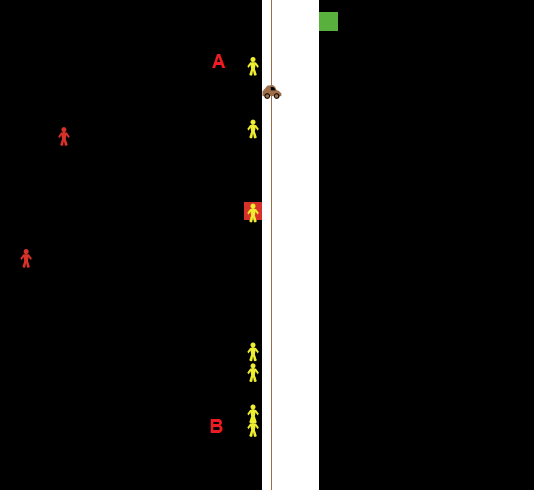
\includegraphics[width=.8\textwidth]{socsim1.png}
\caption{Visualization of the simulation.}
\label{ABlabel}
\end{figure}

If a pedestrian would spot cars on the portion of the road it was watching, it would refuse to cross. As a result, even a moderate amount of cars resulted in pedestrians located at the bottom of the road not crossing when the light was red, regardless of their 'type'.

Additionally, pedestrians standing close to the traffic light would only look ahead a few patches, not noticing cars that might be approaching just behind the traffic light.

\subsubsection{Implementation}
We rewrote the pedestrian's logic such that rather than looking ahead until the traffic light, it would look ahead a fixed number of patches. This 'viewing range would also wrap around the world, meaning the viewing range of pedestrians standing near the top of the road also covered part of the bottom of the road.

\subsubsection{Influences on the simulation}
The area between the bottom of the road and the traffic light was 24 patches high. Consequently, the average viewing range of a pedestrian was about 12 patches.

To quantify the influence of this change on the simulation and its results, we set the viewing range to 8 (picked arbitrarily for testing), and ran the simulation with the exact same parameters as in chapter \ref{sec:initialsim}. The results were:

\begin{table}[H]
\centering
\begin{tabular}{ l | c c c c }
  Police Presence Prob. & 0\% & 33\% & 66\% & 100\% \\ 
  \hline
  Experiment 1 & 3.46 & 2.31 & 0 & 0  \\
  Experiment 2 & 1.83 & 1.31 & 0 & 0  \\
  Experiment 3 & 0.54 & 0.27 & 0 & 0  \\
  Experiment 4 & 0.46 & 0    & 0 & 0  \\
  Experiment 5 & 0.50 & 0    & 0 & 0  \\
  Experiment 6 & 0.13 & 0    & 0 & 0  \\
\end{tabular}
\caption{Average number of times an adaptive 
pedestrian walks through a red light.}
\end{table}

The results for experiments 1 and 4, where no cars were on the road, did not change much, as expected. Interestingly, the results for experiments 2, 3, 5 and 6, when more cars were on the road, increased noticably. 

\subsection{More advanced model}
..

\subsection{Counting methods}
..

\subsection{etc}
..

\clearpage

\section{Simulation}
\subsection{Setup}
Short summary of the setup: parameters, why they were chosen

\subsection{Results}
Short summary of the results of the simulation, perhaps a few remakrs about the differences with the original results.

\clearpage

\section{Conclusion}
Conclusion

\clearpage

\end{document}
